\chapter{Solution}

This chapter describes the complete process of \texttt{Peachpie.Blaozor} functionality, covering the use cases.
It starts with an overview of the library parts.
Then, it gives a detailed description of each part.
\par
\begin{figure}[b!]
\centering
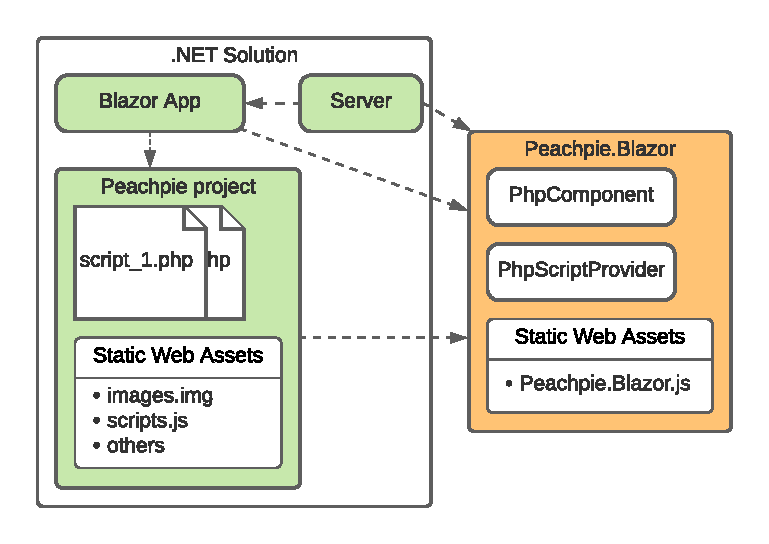
\includegraphics[scale=0.9]{./img/SolutionInfrastructure}
\caption{The .NET solution infrastructure. Green rectangles represent projects. The orange rectangle represents a NuGet package. Arrows represent references.}
\label{img13:infrastructure}
\end{figure} 
\par
\textit{Peachpie.Blazor} is a RCL library containing components mentioned in the previous section with an additional support code.
It is provided as a NuGet package containing an API for including PHP scripts to the website.
It defines a collection of support classes representing HTML entities, which makes the rendering easier.
A part of the support code is a Javascript script, which is linked to the beginning of the HTML document, providing helper functions for form handling and interoperability with PHP.
Then, the resulting Blazor website consists of three projects forming a .NET solution.
In Figure \ref{img13:infrastructure}, we can see these projects as green rectangles.
The \textit{Server} project references \textit{Blazor App}, containing a part of the website, and \textit{Peachpie.Blazor} library, containing the support code.
The server cares about providing the Blazor website and its Static Web Assets.
There is the \textit{Blazor App} project, which becomes the environment for running PHP scripts in a browser.
The rendering process and website composition, where the scripts are evaluated, are meant by the environment.
The project references the Peachpie project containing the programmer's PHP scripts and \textit{Peachpie.Blazor}, which content is used to maintain the scripts.
\textit{Blazor App} inserts the scripts using the components defined in the library.
\par
The first section aims at the server settings providing a Blazor application using PHP scripts and the \textit{Peachpie.Blazor} library.
The second section talks about \texttt{PhpComponent}.
It describes the resulting implementation and solves problems, which occurred during the implementation.
The last section aims at \texttt{PhpScriptProvider}.
It suggests a convenient way how to include the scripts into a browser, and it presents the component design.

\section{Server}

\begin{figure}[b!]
\begin{lstlisting}
{
	...
  "AdditionalStaticWebAssets": [
    {
      "Path": "A//Path//To//Resources//Directory",
      "BasePath": "/Asteroids"
    }
  ]
  ...
}

\end{lstlisting}
\caption{Fragment of configuration file defining additional resources.}
\label{img19:settings}
\end{figure}
\par
The server has to be set in order to provide additional static resources contained in a Peachpie project containing PHP scripts because the WebAssembly SDK ignores the \textit{wwwroot} folder of libraries except for RCL.
Thus, we create the \texttt{UseAdditionalWebStaticAssets} extension method of \texttt{IApplicationBuilder}, which inserts middlewares providing the resources into the request pipeline.
Its parameter is a configuration obtained from \textit{appsettings.json}, which is a part of the \texttt{BlazorApp.Server} project.
We can see an example of the configuration file in Figure \ref{img19:settings}, which defines a path to a folder and a base path used as a prefix of HTML document references.
The path can be absolute or relative to the current working directory.
Afterward, these resources can be referenced by URLs and downloaded from the server.
For example, an HTML document can reference an image with the path \texttt{WebGame/PHPScripts/wwwroot/image.jpg} as \texttt{/Asteroids/image.jpg}.
Javascript helpers of our library can be found in the \textit{wwwroot} folder, which is transparently provided to a client side due to an RCL library type and the SDK.

\section{PhpComponent}

This section introduces several issues caused by many factors, like the difference between the PHP and C\# language.
We analyze these issues and suggest helping concepts, which form the resulting \texttt{PhpComponent} class.
The main objective is to utilize the Peachpie feature allowing to inherit C\# classes, like \texttt{ComponentBase} representing a Blazor component, to provide the full Blazor API in PHP.

\subsection{PhpTreeBuilder}

The first issue is caused by the difference between the PHP and C\# language where Peachpie tries to compensate it, but it is not its main target. 
For example, C\# structs have not a representation in PHP.
Structs are necessary to work with \texttt{RenderTreeBuilder}, which contains API for adding callbacks handling element events, as we can see in Figure \ref{img14:callback}.
This API uses method overloading in many methods.
However, PHP does not support method overloading.
\texttt{AddAttribute} is an example where various types of the attribute value can be passed in.
One of the values can be \texttt{EventCallback} struct representing an event handler.
The struct contains static property \texttt{Factory}, which is a class containing methods for creating callbacks.
\par
\begin{figure}[b!]
\begin{lstlisting}
__builder.OpenElement(5, "button");
__builder.AddAttribute(7, "onclick", 
		EventCallback.Factory.Create<MouseEventArgs>((object)this, 
				(Action)IncrementCount));
__builder.AddContent(8, "Click me");
__builder.CloseElement();
\end{lstlisting}
\caption{Fragment of code adding a button element with an event handler.}
\label{img14:callback}
\end{figure}
\par
Peachpie enables using structs in PHP code. 
However, there are limitations at the time of writing, which force us to make workarounds.
We try to rewrite the previous example in PHP code using Peachpie.
We create a component, which inherits \texttt{ComponentBase}. 
Afterward, we override the method for building a render tree and implement the body.
Peachpie does not allow us to access a static property of struct, which is necessary for obtaining an object providing callbacks representing event callbacks of HTML elements.
Another issue is using a method for creating the callback, which uses many overrides.
Peachpie can not choose the correct version, which results in a runtime error.
We tried to use many workarounds, which used helper classes trying to avoid these issues, but it is impossible to use some Blazor API directly in PHP code.
\par
To make the example working, we can hide the struct from PHP code by implementing a C\# helper method using the struct.
The method should have only parameters compatible with PHP types. 
The overloading can be replaced by a different method name for each overload.
Afterward, Peachpie allows us to call the methods from PHP code.
This approach can be used in the \texttt{AddAtribute} method. 
Defining a new method for each overload is a reasonable approach due to a small number of overloads.
The \texttt{RenderTreeBuilder} does not allow us to inherit it because it is sealed.
For this reason, a wrapper is created containing the builder and defining method for each overload, which calls the original method in C\# code.
This decision leads us to make \texttt{PhpTreeBuilder} wrapping the original builder.

\subsection{Collection of helper classes}

The next issue relates to rendering time.
\texttt{RenderTreeBuilder} provides a method for adding arbitrary markup text.
The text can contain \texttt{<script>}, but its content is not executed.
At first glance, one can see the method as a convenient way to render the whole content, avoiding using other dedicated methods for building the tree.
These methods accept a sequence number used by the diff algorithm. 
Although using the one method for rendering, the whole component causes slow rendering, which is critical in some applications like games.
The diff algorithm relies on marking the blocks of markup by sequence numbers for optimization in page updates.
When there is only one big block, the diff algorithm can not do anything better than generate an update, which renders the whole page. 
This issue can be seen in the Benchmark section comparing the difference between using the one method and utilizing all methods.
\par
Because the builder usage can be complex, we introduce a collection of classes for representing tags, helping implement the code using the builder for rendering.
We present the class diagram in Figure \ref{img16:diagram}.
The main idea is to implement the \texttt{BlazorWritable} interface, which writes the class content into the builder.
An example of the class is \texttt{Tag}, which represents an arbitrary tag.
The tag contains its name, attributes represented by \texttt{AttributeCollection} and inner objects implementing the \texttt{BlazorWritable} interface.
Because a tag can contain other tags using sequence numbers, we have to keep the currently used sequence number used in the diff algorithm.
For this purpose, the \texttt{writeTreeBuilder} method gets the actual sequence number and returns the last unused number.
This API should hide separated class logics for rendering.
The helper classes give a basic implementation of this method, which renders the content with a dynamic sequence numbering. 
However, a programmer can override the method because sequence numbering is impossible to predefine in advance to make the most effective updates.
The next object implementing the interface is the \texttt{Text} class representing a text.
\texttt{AttributeCollection} offers convenient interface for working with attributes by implementing the PHP \texttt{ArrayAccess} interface enabling indexer.
Becuase string values of \texttt{style} and \texttt{class} attributes are more complicated the library provides dedicated classes for working with these attributes, used by \texttt{AttribureCollection}.
\texttt{CssBuilder} and \texttt{ClassBuilder} provide API for creating these values and then format it into the HTML style.
\par
\begin{figure}\centering
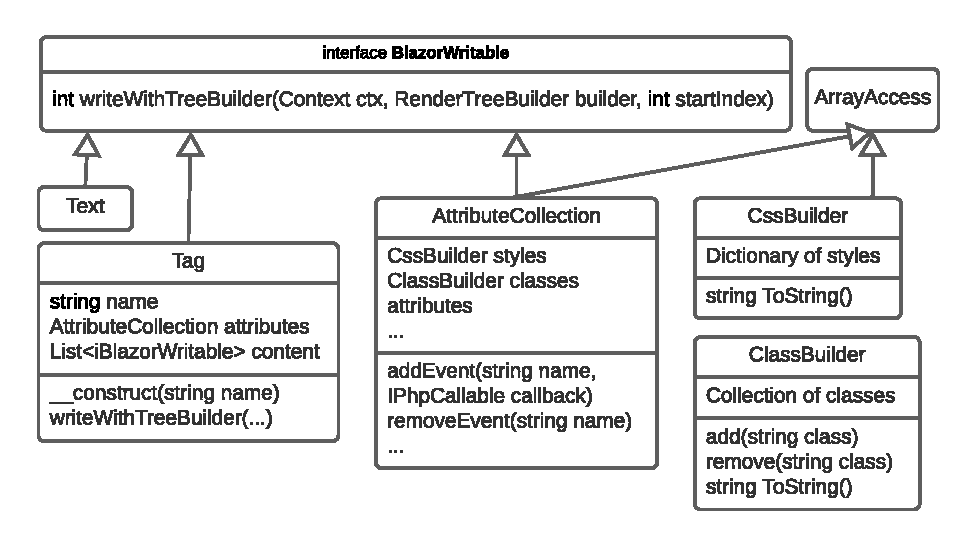
\includegraphics[scale=0.8]{./img/ComponentLibrary}
\caption{Class diagram of supporting library for writting tags.}
\label{img16:diagram}
\end{figure} 
\par
The next barrier is assigning handlers to C\# events in PHP code.
Peachpie does not either support accessing the events.
Thus, a PHP code can not directly use a class like \texttt{Timer}, which is useful in the \textit{WebGame} use case for updating the screen every defined period of time.
The issue can be solved by helper methods defined in a C\# static class, \texttt{EventHelper}.
They accept the object providing some events, handler, and event name.
Afterward, the reflection is used for obtaining the desired event by name from the object and then assign the \texttt{IPhpCallable} handler to it.
Because \texttt{Timer} is a common object, the library contains an additional PHP wrapper class, which uses the timer.
Then a programmer avoids to use the workaround defined above.

\subsection{Interoperability}

The last feature to discuss in this section is interoperability between Javascript and PHP.
Blazor allows calling Javascript functions from C\# \cite{online:interop1} and vice-versa \cite{online:interop2}.
Thus, a Blazor service,\texttt{IJSRuntime} injected by the dispatcher, can be utilized to call Javascript functions.
The service offers a specialized API for that.
Calling PHP from Javascript is more complex.
Peachpie enables calling PHP function by \texttt{Call} method of \texttt{Context}. 
The context finds already defined methods contained in the included PHP script and executes it with the current context.
When we want to call C\# instance method from Javascript, we have to have the reference, supplied by the framework, for calling it.
Additionally, the called C\# method has to be marked with a \texttt{JSInvokableAttribute} during compilation.
The reference can be assigned from C\# by a method, which creates it and uses it as a parameter of a Javascript function.
These conditions lead us to create a new Peachpie context,\texttt{BlazorContext}, which inherits the original Peachpie context and provides the \texttt{CallPHP} method marked by the attribute and calling the PHP function based on parameters.
The context requests the mentioned services provided by the dispatcher and sets the reference by calling predefined code in \texttt{Peachpie.Blazor.js}.
The context will be the Peachpie context of the component.
Thus, it enables to call PHP methods defined in this context from Javascript by using the reference.
The advantage of this approach is that there can be two components inheriting \texttt{PhpComponent} with the same context when their context is set to the same instance.
Thus, we can call their functions only by one reference.

\subsection{Summary}

\begin{figure}[t!]
\centering
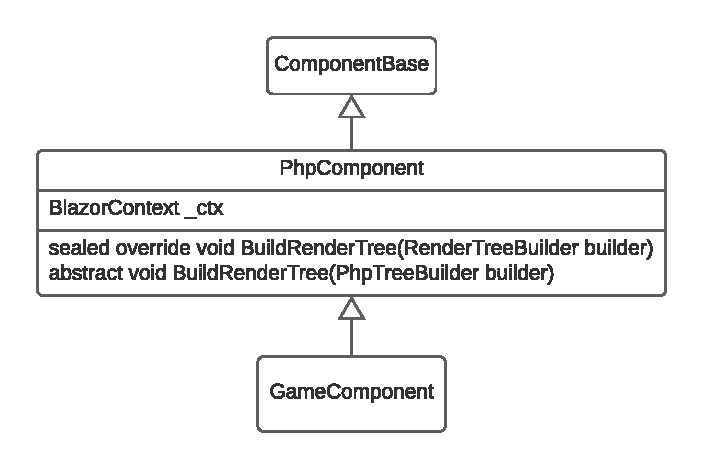
\includegraphics[scale=0.8]{./img/PhpComponentSolution}
\caption{Class diagram of the use case implementation.}
\label{img17:solution}
\end{figure}
\par
This section summarizes the architecture of \texttt{PhpComponent} and main implementation idea of \textit{WebGame} use case.
The component hides the original function for rendering and replaces it with our version of the builder, as shown in Figure \ref{img17:solution}.
It results in transparent usage of the builder in the inherited class.
The builder is just a wrapper, so the programmer can use the original builder by accessing its property, \texttt{Builder}.
Additionally, there is a collection of classes for creating tags, making builder usage easier.
For assigning PHP handlers to C\# events, there is a universal helper class, \texttt{EventHelper}.
Furthermore, the last feature is a timer wrapper, which uses the C\# timer, offering a convenient API.
Interoperability with Javascript is provided by our predefined API using \texttt{BlazorContext}.
These features are sufficient for implementing a game described in \textit{WebGame} use case.
Using PHP functions as handlers, the timer is used to update the game screen by \texttt{StateHasChanged}.
The update consists of evaluating the position of game entities, which use the helper classes representing HTML entities.
Lastly, context preservation is used to keep the game state.
\par
The last necessary thing is to pass assembly references containing the components into \texttt{Router}, which is a standard duty in Blazor.

\section{PhpScriptProvider}

The beginning of this section introduces the main component parts, which gives us an overview of the component composition.
Component duties like navigation or script execution are divided into subsections because the component consists of many processes, which are complex to describe at once in the structure.
The component functionality will be explained in these sections.
\par
\begin{figure}[b!]
\centering
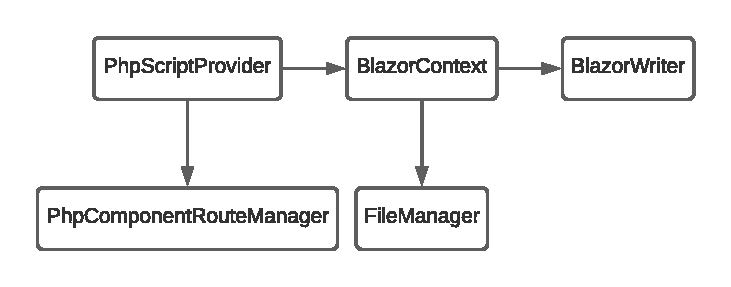
\includegraphics[scale=0.8]{./img/PhpScriptProvider}
\caption{Diagram illustrating usage of PhpScriptProvider main parts.}
\label{img18:provider}
\end{figure}
\par
Figure \ref{img18:provider} describes the connections between the main parts.
\texttt{PhpScriptProvider} is a class, representing a Blazor component.
The component manages the following features.
\par
\begin{itemize}
\item It handles the navigation.
\item It finds the script by name based on provider mode.
\item It creates and keeps a PHP context, which is used for script execution.
\item It executes the script.
\end{itemize}
\par
These duties contain several steps, which are maintained by the helper classes.
As we can see, there is \texttt{PhpComponentRouteManager}, which finds the components, inheriting \texttt{PhpComponent}, based on \texttt{RouteAttribute}.
It enables navigation of Blazor components defined in PHP scripts.
The next part is \texttt{BlazorContext} already mentioned in PhpComponent, which is Peachpie \texttt{Context} designed for Blazor enviroment.
The context constructor accepts several Blazor services like \texttt{IJSRuntime} enabling interoperability with Javascript.
The context initializes superglobals based on URL and submitted forms, manages files uploaded by a form, and controls  \texttt{BlazorWriter} which redirects the script output to the render tree.
Lastly, \texttt{FileManager} reads submitted files, downloads them, or deletes them from Browser memory.
\par
The following paragraph zooms in \texttt{PhpScriptProvider} structure in order to better understand processes maintaining the features.
The provider contains of many properties.
Some of them are injected by the dispatcher like \texttt{NavigationManager} or \texttt{IJSRuntime}, which is a service providing interoperability with Javascript.
Others can be parametrized, like \texttt{Type} determining the mode of provider, \texttt{ContextLifetime} determining the persistency of the script context, or \texttt{ScriptName} determining the executing script when the mode \textit{Script} is set.
These properties influence the component methods.
The first method is \texttt{Attach}, which assigns a render handle providing \texttt{RenderTreeBuilder}, and registers a navigation handler creating the context and calling \texttt{Refresh}.
The second method,\texttt{SetParameters}, handles calling \texttt{Refresh}, and creating the context as well.
\texttt{Refresh} finds a script or a component based on properties, assigns the superglobals, and calls \texttt{Render} which renders the component or executes the script.
\texttt{OnAfterRender} cares about enabling the forms to send data back to Blazor.
Some of these methods are called by Blazor framework providing the component lifecycle.

\subsection{Navigation}

The section explains navigation in \texttt{PhpScriptProvider} for each of provider modes.
We have to clarify how the component is instantiated and maintained by Blazor.
There are two ways how to use the component.
The first of them is to set it in \texttt{WebAssemblyBuilder} as a root component,
which is rendered after the first application launch in Blazor.
The component is alive for the whole application life because there is no \texttt{Router}, which disposes components representing a previous page. 
It results in calling the \texttt{Attach} method and the \texttt{SetParameters} method only once.
The second way is to use a Razor page containing the component and let the navigation to the page on \texttt{Router}, which is a root component by default.
When the page is navigated, the component is instantiated as well.
The difference is the possibility of calling the \texttt{SetParameters} method multiple times when the page is parameterized.
Then, when the parameters are changed, Blazor automatically calls the inner component \texttt{SetParameters} methods if the components have at least one complex type. 
This fact is because the Blazor framework can not decide if the parameters, which are complex types, were changed.
\par
The \textit{Router} mode is designed to be used when the component is a root component.
Then, it is certain that \texttt{Attach} and \texttt{SetParameters} methods are called only once.
Thus, navigation handler is registered in the \texttt{Attach} method, which should handle further navigation.
When the navigation occurs, a new context is created if the context should not be persistent, then the \texttt{Refresh} method is called.
\texttt{SetParameters} creates a new context and calls the \texttt{Refresh} method as well, but the method is called only once at the beginning of the application.
Then the \texttt{Refresh} method parses the query part of URL \cite{online:querryStrings}, obtained from \texttt{NavigationManager} and gets the script name from the URL.
When the script name is determined, the method calls the \texttt{Render} method, where it decides if it is a script or a component defined in a script based on \texttt{.php} extension.
If the extension is missing, it tries to find a component defined in scripts, which has correct \texttt{RouteAttribute} by \texttt{PhpComponentRouteManager}.
Otherwise, it asks the Peachpie context for obtaining the script representation as \texttt{ScriptInfo}.
Additional manager duty is to assign assembly references containing scripts, to the context, at the beginning of the application.
The context does not have to know the script name, or the component does not have to exist. 
Then, the \texttt{Render} method renders predefined \textit{not found} page, which can be set by \texttt{PhpScriptProvider} parameters.
Otherwise, it renders the script or the component.
Additionally, when the component is navigated, the method sets its context by the current provider context.
It results in using the interoperability by either provider or the component because there is the same context reference in Javascript code.
\par
Next modes, \textit{ScriptProvider} and \textit{Script}, are similar.
They are defined in a Razor page and initialized when the page is navigated.  
The difference is finding the script by name, where the \textit{Script} always uses the name defined in the component parameter and \textit{ScriptProvider} finds script based on URL.
As we said, the \texttt{SetParameters} can be called multiple times, so the method calls \texttt{Refresh} only by the first time.
Additional rendering is initiated by the navigation handler.
Thus, when the navigation occurs, it finds and update the page, or the component is disposed if \texttt{Router} matches another Razor page.
A new context is created based on the \texttt{ContextLifetime} mode.
It differs from common PHP behavior, where the context is disposed after scritps handles the request.
This unusual approach allows calling functions defined in the context after the component is rendered, which is a part of Javascript interoperability when PHP functions can by called by Javascript.
We should check if the component has not already been disposed by \texttt{Router} before calling the \texttt{Refresh}.
Obtaining the script is similar to \textit{Router} mode.

\subsection{Script Execution}

We start with \texttt{BlazorWriter}, which inherits \texttt{TextWriter}.
The inheritance allows using the writer as \texttt{BlazorContext} output writer, which manipulates with script output.
The writer consists of a buffer and \texttt{RenderTreeBuilder}.
The main usage is to write any string to the writer, which adds it to the buffer.
In the end, the writer flushes it into the builder by \texttt{AddMarkUpContent}.
It results in treating the whole script output as one modification by diff algorithm, which causes the whole page update instead of smaller necessary updates.
This approach is chose due to the following limitations.
\texttt{AddMarkUpContent} does not allow to add incomplete markup text, meaning that tags are not properly closed.
Thus, we can not divide the text into smaller parts because of the HTML nature, where tags are coupled by other tags.
The second possibility is to parse the output and recognize the types of HTML entities, which can use specialized builder API.
However, it is not suitable because of parser complexity.
It is important to dispose the writer after the rendering because the same builder can not be repeatedly used.
\par
\texttt{BlazorContext} maintains the writer and interoperability with Javascript.
It provides methods for initializing and ending the rendering.
The script represented by \texttt{ScriptInfo} is executed by its method \texttt{Evaluate}. This method accepts the context, which maintains the script output by redirecting it to the render tree.
It also allows setting superglobals like \texttt{\$\_GET} to provide the query part of URL and turns forms to client-side 
handling, which is described in the following section.

\subsection{Forms}

Typically, web forms are not handled by Blazor, and the are sent to the server.
Javascript interoperability is used to evaluate them on the client side.
It starts in \texttt{AfterRender} method, where it calls our Javascript function, which finds all already rendered forms and assigns them an event handler for submitting.
When submit occurs, the handler collects all data from the form, does ordinary navigation to the page defined in \texttt{action} attribute, and prevents default behavior, which is sending the form to the server.
When the navigation is handled by \texttt{PhpScriptProvider}, it gets all collected data and assigns the context superglobals by them.
Afterward, the script is executed, and it can access the superglobals.
\par
The previous paragraph did not explain the file management due to its complexity.
We describe it now.
When a user loads files by form, Javascript obtains only the list of files. 
When a programmer wants to read the content, he or she has to use a reading operation, which is done asynchronously by \texttt{Promise} mentioned in the Javascript section.
Thus, when we get the data during navigation, the page rendering has to wait until the content is read.
This operation could take a long time, so the page shows old content.
For this reason, we provide an additional parameter for defining the content, which is shown during navigation.
An alternative is initializing reading by a PHP script when it is executed.
It uses interoperability between PHP, C\#, and Javascript in order to call desired reading methods.
Unfortunately, Blazor does not allow us to wait until the reading operation is done, and we have to provide callbacks, which handle the end of the reading.
We suppose that it is confusing for potential PHP programmers, who will use \texttt{Peachpie.Blazor} to define PHP callbacks.
We decide to prefetch the file content before the execution to provide the data synchronously in PHP code.
\par
Interoperability in the provider can be achieved in a similar manner as in \texttt{PhpComponent}.
The difference is calling the Javascript functions, which use prefined API using our context, which uses the \texttt{IJSRuntime} service.

\section{Templates}

A \ac{VS} template is a prepared project or collection of projects, which is adjusted by a programmer.
This approach of creating a new software is comfortable for the user because he or she does not have to start with an empty folder.
We created templates for VS 2019 in order to make the website creating easier.
The templates are copied and adjusted from Peachpie templates \cite{online:templates} and comprise the first and the third example, presented in the following section, packed into a NuGet package.
Usage and compilation of templates can be found in the attachments.
 